\documentclass{amsart}
% !TEX root = ../msimplicial.tex

\usepackage{microtype}
\usepackage{amssymb}
\usepackage{mathtools}
\usepackage{tikz-cd}
\usepackage{mathbbol} % changes \mathbb{} and adds more support

% bibliography
\usepackage[
	backend=biber,
	style=alphabetic,
	backref=true,
	url=false,
	doi=false,
	isbn=false,
	eprint=false]{biblatex}

\renewbibmacro{in:}{}  % don't display "in:" before the journal name
\AtEveryBibitem{\clearfield{pages}}  % don't show page numbers

\DeclareFieldFormat{title}{\myhref{\mkbibemph{#1}}}
\DeclareFieldFormat
[article,inbook,incollection,inproceedings,patent,thesis,unpublished]
{title}{\myhref{\mkbibquote{#1\isdot}}}

\newcommand{\doiorurl}{%
	\iffieldundef{url}
	{\iffieldundef{eprint}
		{}
		{http://arxiv.org/abs/\strfield{eprint}}}
	{\strfield{url}}%
}

\newcommand{\myhref}[1]{%
	\ifboolexpr{%
		test {\ifhyperref}
		and
		not test {\iftoggle{bbx:eprint}}
		and
		not test {\iftoggle{bbx:url}}
	}
	{\href{\doiorurl}{#1}}
	{#1}%
}

% references
\usepackage[
	bookmarks=true,
	linktocpage=true,
	bookmarksnumbered=true,
	breaklinks=true,
	pdfstartview=FitH,
	hyperfigures=false,
	plainpages=false,
	naturalnames=true,
	colorlinks=true,
	pagebackref=false,
	pdfpagelabels]{hyperref}

\hypersetup{
	colorlinks,
	citecolor=blue,
	filecolor=blue,
	linkcolor=blue,
	urlcolor=blue
}

\usepackage[capitalize, noabbrev]{cleveref}
\let\subsectionSymbol\S
\crefname{subsection}{\subsectionSymbol\!}{subsections}

% layout
\addtolength{\textwidth}{0in}
\addtolength{\textheight}{0in}
\calclayout

% update to MSC2020
\makeatletter
\@namedef{subjclassname@2020}{%
	\textup{2020} Mathematics Subject Classification}
\makeatother

% table of contents
\setcounter{tocdepth}{1}

% !TEX root = ../msimplicial.tex

\newcommand{\mSet}{\mathsf{mSet}}
\newcommand{\stspx}[1]{\simplex^{\!#1}}
\newcommand{\msimplex}[1]{\simplex^{\!\times\mathit{#1}}}
\newcommand{\dsimplex}{\simplex^{n_1} \times \dots \times \simplex^{n_k}}

\DeclareMathOperator{\cU}{\mathcal{U}}
\DeclareMathOperator{\fM}{\mathfrak{M}}
\DeclareMathOperator{\cs}{\mathfrak{cs}}
\DeclareMathOperator{\ez}{\mathfrak{ez}}
\DeclareMathOperator{\CS}{CS}

\DeclareMathOperator{\schainsUM}{N^{\simplex}_{\UM}}
\DeclareMathOperator{\mchainsk}{\chains^{\msimplex{k}}}
\DeclareMathOperator{\mchainskUM}{\chains^{\msimplex{k}}_{\UM}}
\DeclareMathOperator{\copr}{\Delta}
\DeclareMathOperator{\aug}{\epsilon}
\DeclareMathOperator{\pr}{\ast}
\DeclareMathOperator{\sh}{\mathfrak{sh}}

\newcommand{\paolo}[1]{\textcolor{green}{\underline{Paolo}: #1}}
\newcommand{\andrea}[1]{\textcolor{yellow}{\underline{Andrea}: #1}}

\title[Short title]{Multisimplicial cochain operations}

\author[A. Medina-Mardones]{Anibal M. Medina-Mardones}
\address{A.M-M., Max Planck Institute for Mathematics \and University of Notre Dame}
\email{\href{mailto:ammedmar@mpim-bonn.mpg.de}{ammedmar@mpim-bonn.mpg.de}}

\author[A. Pizzi]{Andrea Pizzi}
\address{Dipartimento di Matematica "Giuseppe Peano", Universit\`a degli studi di Torino} 
\email{andrea.pizzi@edu.unito.it}

\author[P. Salvatore]{Paolo Salvatore}
\address{Dipartimento di Matematica, Universit\`a di Roma Tor Vergata} 
\email{salvator@mat.uniroma2.it}

\date{\today}
\subjclass[2020]{.}
\keywords{.}

\usetikzlibrary{arrows,decorations.markings}
\tikzset{myptr/.style={decoration={markings,mark=at position 1 with %
			{\arrow[scale=2,>=stealth]{>}}},postaction={decorate}}}

\newsavebox\preproduct
\begin{lrbox}{\preproduct}
	\begin{tikzpicture}[scale=.3]
	\draw (0,0)--(0,-.8);
	\draw (0,0)--(.5,.5);
	\draw (0,0)--(-.5,.5);
	\end{tikzpicture}
\end{lrbox}
\newcommand{\product}{% <- this 'right of' is inherited; how to avoid?
	\usebox\preproduct}

\newsavebox\precoproduct
\begin{lrbox}{\precoproduct}
	\begin{tikzpicture}[scale=.3]
	\draw (0,0)--(0,.8);
	\draw (0,0)--(.5,-.5);
	\draw (0,0)--(-.5,-.5);
	\end{tikzpicture}
\end{lrbox}
\newcommand{\coproduct}{% <- this 'right of' is inherited; how to avoid?
	\usebox\precoproduct}

\newsavebox\preboundary
\begin{lrbox}{\preboundary}
	\begin{tikzpicture}[scale=.3]
	\draw (0,0)--(0,1.3);
	\draw (.5,0)--(.5,1.3);
	\draw [fill] (0,0) circle [radius=0.1];
	\draw (.9,.6)--(1.3,.6);
	\draw (1.7,0)--(1.7,1.3);
	\draw (2.2,0)--(2.2,1.3);
	\draw [fill] (2.2,0) circle [radius=0.1];
	\end{tikzpicture}
\end{lrbox}
\newcommand{\boundary}{% <- this 'right of' is inherited; how to avoid?
	\usebox\preboundary}

\newsavebox\preleftboundary
\begin{lrbox}{\preleftboundary}
	\begin{tikzpicture}[scale=.3]
	\draw (1.7,0)--(1.7,1.3);
	\draw (2.2,0)--(2.2,1.3);
	\draw [fill] (2.2,0) circle [radius=0.1];
	\end{tikzpicture}
\end{lrbox}
\newcommand{\leftboundary}{% <- this 'right of' is inherited; how to avoid?
	\usebox\preleftboundary}

\newsavebox\prerightboundary
\begin{lrbox}{\prerightboundary}
	\begin{tikzpicture}[scale=.3]
	\draw (0,0)--(0,1.3);
	\draw (.5,0)--(.5,1.3);
	\draw [fill] (0,0) circle [radius=0.1];
	\end{tikzpicture}
\end{lrbox}
\newcommand{\rightboundary}{% <- this 'right of' is inherited; how to avoid?
	\usebox\prerightboundary}

\newsavebox\precoboundary
\begin{lrbox}{\precoboundary}
	\begin{tikzpicture}[scale=.3]
	\draw (0,0)--(0,1.3);
	\draw (.5,0)--(.5,1.3);
	\draw [fill] (0,1.3) circle [radius=0.1];
	\draw (.9,.6)--(1.3,.6);
	\draw (1.7,0)--(1.7,1.3);
	\draw (2.2,0)--(2.2,1.3);
	\draw [fill] (2.2,1.3) circle [radius=0.1];
	\end{tikzpicture}
\end{lrbox}
\newcommand{\coboundary}{% <- this 'right of' is inherited; how to avoid?
	\usebox\precoboundary}

\newsavebox\precounit
\begin{lrbox}{\precounit}
	\begin{tikzpicture}[scale=.3]
	\draw (0,0)--(0,1.3);
	\draw [fill] (0,0) circle [radius=0.1];
	\end{tikzpicture}
\end{lrbox}
\newcommand{\counit}{% <- this 'right of' is inherited; how to avoid?
	\usebox\precounit}

\newsavebox\preidentity
\begin{lrbox}{\preidentity}
	\begin{tikzpicture}[scale=.3]
	\draw (0,0)--(0,1.3);
	\end{tikzpicture}
\end{lrbox}
\newcommand{\identity}{% <- this 'right of' is inherited; how to avoid?
	\usebox\preidentity}

\newsavebox\preunit
\begin{lrbox}{\preunit}
	\begin{tikzpicture}[scale=.3]
	\draw (0,0)--(0,1.3);
	\draw [fill] (0,1.3) circle [radius=0.1];
	\end{tikzpicture}
\end{lrbox}
\newcommand{\unit}{% <- this 'right of' is inherited; how to avoid?
	\usebox\preunit}

\newsavebox\preassociativity
\begin{lrbox}{\preassociativity}
	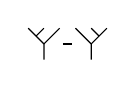
\begin{tikzpicture}[scale=.2]
	\path[draw] (0,0)--(0,1)--(-1,2);
	\draw (0,1)--(1,2);
	\draw (-.5,1.5)--(0,2);
	\draw (1.2,1)--(1.8,1);
	\path[draw] (3,0)--(3,1)--(2,2);
	\draw (3,1)--(4,2);
	\draw (3.5,1.5)--(3,2);
	\end{tikzpicture}
\end{lrbox}
\newcommand{\associativity}{% <- this 'right of' is inherited; how to avoid?
	\usebox\preassociativity}

\newsavebox\precoassociativity
\begin{lrbox}{\precoassociativity}
	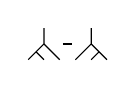
\begin{tikzpicture}[scale=.2]
	\path[draw] (0,0)--(0,-1)--(-1,-2);
	\draw (0,-1)--(1,-2);
	\draw (-.5,-1.5)--(0,-2);
	\draw (1.2,-1)--(1.8,-1);
	\path[draw] (3,0)--(3,-1)--(2,-2);
	\draw (3,-1)--(4,-2);
	\draw (3.5,-1.5)--(3,-2);
	\end{tikzpicture}
\end{lrbox}
\newcommand{\coassociativity}{% <- this 'right of' is inherited; how to avoid?
	\usebox\precoassociativity}

\newsavebox\preleftcomb
\begin{lrbox}{\preleftcomb}
	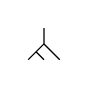
\begin{tikzpicture}[scale=.2]
	\path[draw] (0,0)--(0,-1)--(-1,-2);
	\draw (0,-1)--(1,-2);
	\draw (-.5,-1.5)--(0,-2);
	\end{tikzpicture}
\end{lrbox}
\newcommand{\leftcomb}{% <- this 'right of' is inherited; how to avoid?
	\usebox\preleftcomb}

\newsavebox\prerightcomb
\begin{lrbox}{\prerightcomb}
	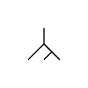
\begin{tikzpicture}[scale=.2]
	\path[draw] (3,0)--(3,-1)--(2,-2);
	\draw (3,-1)--(4,-2);
	\draw (3.5,-1.5)--(3,-2);
	\end{tikzpicture}
\end{lrbox}
\newcommand{\rightcomb}{% <- this 'right of' is inherited; how to avoid?
	\usebox\prerightcomb}

\newsavebox\preinvolution
\begin{lrbox}{\preinvolution}
	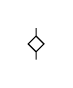
\begin{tikzpicture}[scale=.2]
	\path[draw] (0,0)--(0,.5)--(-.5,1)--(0,1.5)--(0,2);
	\path[draw] (0,.5)--(.5,1)--(0,1.5);
	\end{tikzpicture}
\end{lrbox}
\newcommand{\involution}{% <- this 'right of' is inherited; how to avoid?
	\usebox\preinvolution}

\newsavebox\preleftcounitality
\begin{lrbox}{\preleftcounitality}
	\begin{tikzpicture}[scale=.3]
	\draw (0,0)--(0,.8);
	\draw (0,0)--(.5,-.5);
	\draw (0,0)--(-.5,-.5);
	\draw [fill] (-.5,-.5) circle [radius=0.1];
	\draw (.7,0)--(1.1,0);
	\path[draw] (1.5,-.5)--(1.5,.8);
	\end{tikzpicture}
\end{lrbox}
\newcommand{\leftcounitality}{% <- this 'right of' is inherited; how to avoid?
	\usebox\preleftcounitality}

\newsavebox\preleftcounitcoproduct
\begin{lrbox}{\preleftcounitcoproduct}
	\begin{tikzpicture}[scale=.3]
	\draw (0,0)--(0,.8);
	\draw (0,0)--(.5,-.5);
	\draw (0,0)--(-.5,-.5);
	\draw [fill] (-.5,-.5) circle [radius=0.1];
	\end{tikzpicture}
\end{lrbox}
\newcommand{\leftcounitcoproduct}{% <- this 'right of' is inherited; how to avoid?
	\usebox\preleftcounitcoproduct}

\newsavebox\prerightcounitality
\begin{lrbox}{\prerightcounitality}
	\begin{tikzpicture}[scale=.3]
	\draw (0,0)--(0,.8);
	\draw (0,0)--(.5,-.5);
	\draw (0,0)--(-.5,-.5);
	\draw [fill] (.5,-.5) circle [radius=0.1];
	\draw (-.7,0)--(-1.1,0);
	\path[draw] (-1.5,-.5)--(-1.5,.8);
	\end{tikzpicture}
\end{lrbox}
\newcommand{\rightcounitality}{% <- this 'right of' is inherited; how to avoid?
	\usebox\prerightcounitality}

\newsavebox\prerightcounitcoproduct
\begin{lrbox}{\prerightcounitcoproduct}
	\begin{tikzpicture}[scale=.3]
	\draw (0,0)--(0,.8);
	\draw (0,0)--(.5,-.5);
	\draw (0,0)--(-.5,-.5);
	\draw [fill] (.5,-.5) circle [radius=0.1];
	\end{tikzpicture}
\end{lrbox}
\newcommand{\rightcounitcoproduct}{% <- this 'right of' is inherited; how to avoid?
	\usebox\prerightcounitcoproduct}

\newsavebox\preleftunitality
\begin{lrbox}{\preleftunitality}
	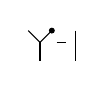
\begin{tikzpicture}[scale=.3]
	\draw (0,0)--(0,-.8);
	\draw (0,0)--(-.5,.5);
	\draw (0,0)--(.5,.5);
	\draw [fill] (.5,.5) circle [radius=0.1];
	\draw (.7,0)--(1.1,0);
	\path[draw] (1.5,.5)--(1.5,-.8);
	\end{tikzpicture}
\end{lrbox}
\newcommand{\leftunitality}{% <- this 'right of' is inherited; how to avoid?
	\usebox\preleftunitality}

\newsavebox\prerightunitality
\begin{lrbox}{\prerightunitality}
	\begin{tikzpicture}[scale=.3]
	\draw (0,0)--(0,-.8);
	\draw (0,0)--(-.5,.5);
	\draw (0,0)--(.5,.5);
	\draw [fill] (-.5,.5) circle [radius=0.1];
	\draw (-.7,0)--(-1.1,0);
	\path[draw] (-1.5,.5)--(-1.5,-.8);
	\end{tikzpicture}
\end{lrbox}
\newcommand{\rightunitality}{% <- this 'right of' is inherited; how to avoid?
	\usebox\prerightunitality}

\newsavebox\preproductcounit
\begin{lrbox}{\preproductcounit}
	\begin{tikzpicture}[scale=.3]
	\draw (0,0)--(0,-.8);
	\draw (0,0)--(.5,.5);
	\draw (0,0)--(-.5,.5);
	\draw [fill] (0,-.8) circle [radius=0.1];
	\end{tikzpicture}
\end{lrbox}
\newcommand{\productcounit}{% <- this 'right of' is inherited; how to avoid?
	\usebox\preproductcounit}

\newsavebox\preunitcoproduct
\begin{lrbox}{\preunitcoproduct}
	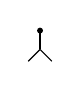
\begin{tikzpicture}[scale=.3]
	\draw (0,0)--(0,.8);
	\draw (0,0)--(.5,-.5);
	\draw (0,0)--(-.5,-.5);
	\draw [fill] (0,.8) circle [radius=0.1];
	\end{tikzpicture}
\end{lrbox}
\newcommand{\unitcoproduct}{% <- this 'right of' is inherited; how to avoid?
	\usebox\preunitcoproduct}

\newsavebox\preleibniz
\begin{lrbox}{\preleibniz}
	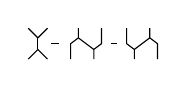
\begin{tikzpicture}[scale=.245]
	\draw (0,.3)--(0,-.3);
	\draw (0,.3)--(.5,.8);
	\draw (0,.3)--(-.5,.8);
	\draw (0,-.3)--(0,.3);
	\draw (0,-.3)--(.5,-.8);
	\draw (0,-.3)--(-.5,-.8);

	\draw (.7,0)--(1.1,0);
	\draw (2.1,.8)--(2.1,.3)--(1.7,0)--(1.7,-.8);
	\draw (2.1,.3)--(2.9,-.3);
	\draw (3.3,.8)--(3.3,0)--(2.9,-.3)--(2.9,-.8);

	\draw (3.8,0)--(4.1,0);
	\draw (4.6,.8)--(4.6,0)--(5,-.3)--(5,-.8);
	\draw (5,-.3)--(5.8,.3);
	\draw (5.8,.8)--(5.8,.3)--(6.2,0)--(6.2,-.8);
	\end{tikzpicture}
\end{lrbox}
\newcommand{\leibniz}{% <- this 'right of' is inherited; how to avoid?
	\usebox\preleibniz}

\newsavebox\prebialgebra
\begin{lrbox}{\prebialgebra}
	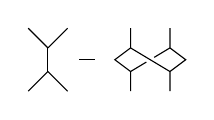
\begin{tikzpicture}[scale=.5]
	\draw (0,.3)--(0,-.3);
	\draw (0,.3)--(.5,.8);
	\draw (0,.3)--(-.5,.8);
	\draw (0,-.3)--(0,.3);
	\draw (0,-.3)--(.5,-.8);
	\draw (0,-.3)--(-.5,-.8);

	\draw (.8,0)--(1.2,0);

	\draw (2.1,.8)--(2.1,.3)--(1.7,0)--(2.1,-.3)--(2.1,-.8);

	\draw (3.1,.8)--(3.1,.3)--(3.5,0)--(3.1,-.3)--(3.1,-.8);

	\draw (2.1,.3)--(3.1,-.3);
	\draw (2.1,-.3)--(2.5,-.06);
	\draw (3.1,.3)--(2.7,.06);
	\end{tikzpicture}
\end{lrbox}
\newcommand{\bialgebra}{% <- this 'right of' is inherited; how to avoid?
	\usebox\prebialgebra}

\newsavebox\precommutativity
\begin{lrbox}{\precommutativity}
	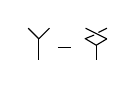
\begin{tikzpicture}[scale=.27]
	\draw (.3,0)--(.3,-1);
	\draw (.3,0)--(.8,.5);
	\draw (.3,0)--(-.2,.5);

	\draw (1.2,-.4)--(1.8,-.4);

	\draw (3,-.3)--(3,-1);
	\draw (2.5,0)--(3,-.3);
	\draw (3.5,0)--(3,-.3);
	\draw (2.46,0)--(2.9,.18);
	\draw (3.1,.3)--(3.5,.5);
	\draw (3.5,0)--(2.5,.5);
	\end{tikzpicture}
\end{lrbox}
\newcommand{\commutativity}{% <- this 'right of' is inherited; how to avoid?
	\usebox\precommutativity}

\begin{document}
	
\begin{abstract}
	
\end{abstract}
	\maketitle
	% !TEX root = ../msimplicial.tex

\section{Introduction}\todo{@everyone: to be updated.} \label{s:introduction}

The normalized cochain complex $N^*(K)$ of a simplicial set $K$ is equipped with the classical Alexander-Whitney cup product that makes into a differential graded algebra.
Our first goal is to extend this product to the case of multisimplicial sets.  Let us consider a $k$-fold simplicial set $X$, that is a contravariant functor from $(\Delta)^k$ to the category of sets. The restriction to the diagonal  $\Delta \subset (\Delta)^k$ defines a simplicial set $X^D$. There is a notion
of geometric realization $|X|$ of a $k$-fold simplicial set $X$, that is a CW complex with a cell $e_x$ for each non-degenerate multisimplex $x$, with a characteristic map from a product of simplexes  $$\Delta_{i_1} \times \dots \times \Delta_{i_k} \to e_x$$ This extends the classical case where the characteristic map has a single simplex as domain.
Quillen proved in
\cite{Quillen} that there is  a natural homeomorphism of realizations $|X| \cong |X^D|$. Under this homeomorphism the cells of $|X^D|$ arise from those
of $|X|$ by subdividing $k$-fold products of simplexes into simplexes. This procedure is described combinatorially by the Eilenberg-Zilber quasi-isomorphism $$EZ:N_*(X) \to N_*(X^D)$$

%that induces a quasi-isomorphism on normalized chains
%$N_*(X) \to N_*(X^D)$ after quotienting out degenerate %chains.
% As in the classical simplicial case, the projection $C_*(X) \to N_*(X)$ onto normalized chains
%is a quasi-isomorphism.

\medskip

 We prove in Theorem \ref{algebra}  %quale?
 that the cochain complex $N^*(X)$ is equipped with a differential graded algebra structure.
 The product is the natural extension to the multisimplicial case of the cup product  defined by the Alexander-Whitney formula, by
  evaluating cochains on front and rear faces in all multisimplicial directions. %formula?
  We prove in section \ref{ultima}
   that the dual Eilenberg-Zilber map
 $$EZ^*:N^*(X^D) \to N^*(X)$$ %provato dove?
  is a quasi-isomorphism of differential graded algebras, where the source is equipped with the classical cup product.
We extend the previous construction to an $E_\infty$ structure on multisimplicial cochains using the approach defined by the first author in \cite{anibal}.
In this case $EZ$ does not respect the $E_\infty$-structures, but there is a natural quasi-isomorphism in the opposite direction that does preserve them.
\paolo{anibal elaborates on Cartan-Serre?}

 Our result is very useful for computations, since multisimplicial models of spaces have a significantly smaller number of non-degenerate cells then their simplicial models.
So $N^*(X)$ is much smaller than $N^*(X^D)$, but it contains the same information up to homotopy,
allowing for example
to calculate explicitly homology operations like Massey products, and the Steenrod algebra action.
As an example we consider a family of multisimplicial sets $Sur(k)$ defined  by McClure and Smith, see \cite{MS},  modelling euclidean configuration spaces.
The proof by the third author of the non-formality of the cochain algebra of planar configuration spaces in \cite{formality}  used the Barratt-Eccles simplicial model and the classical cup product.
Our new product on the multisimplicial McClure-Smith models makes the computation much simpler and faster, paving the way for an extension to higher dimensions.
%per esempio dire i numeri..

\medskip

Part of the results appeared in the B.Sc. thesis of the second author, University of Rome Tor Vergata (2019), written under the guidance of the third author.
	
\subsection*{Acknowledgment}
	% !TEX root = ../msimplicial.tex

\section{Conventions and preliminaries} \label{s:preliminaries}

\subsection{Chain complexes }

Throughout this article $\k$ denotes a commutative and unital ring and we work over its associated closed symmetric monoidal category of differential (homologically) graded $\k$-modules $(\Ch, \ot, \k)$.
We refer to the objects and morphisms of this category as \textit{chain complexes} and \textit{chain maps} respectively. We denote by $\Hom(C, C^\prime)$ the chain complex of $\k$-linear maps between chain complexes $C$ and $C^\prime$, and refer to the functor $\Hom(-, \k)$ as \textit{linear duality}.

\anibal{Be more explicit about tensor product and the closed monoidal property}

\subsection{Category theory}

%A category is said to be \textit{Cartesian} if is a monoidal category whose monoidal structure is given by the category-theoretic product and whose unit is a terminal object.
%A Cartesian category $(\mathsf{A}, \times, \mathbb{1})$ is equipped with natural diagonal and augmentation maps $\Delta_a \colon a \to a \times a$ and $\varepsilon_a \colon a \to \mathbb{1}$.
%
%\anibal{maybe this notion is not needed}

Recall that a category is said to be \textit{small} if its objects and morphisms form sets.
We denote the Cartesian category of small categories by $\Cat$.

Given categories $\sB$ and $\sC$ we denote their associated \textit{functor category} by $\Fun(\sB, \sC)$.

A category is said to be \textit{cocomplete} if any functor to it from a small category has a colimit.
If $\mathsf{A}$ is small and $\mathsf{C}$ cocomplete, then the (left) \textit{Kan extension of $g$ along $f$} exists for any pair of functors $f$ and $g$ in the diagram below, and it is the initial object in $\Fun(\sB, \mathsf{C})$ making
\begin{equation*}
\begin{tikzcd}[column sep=normal, row sep=normal]
\mathsf{A} \arrow[d, "f"'] \arrow[r, "g"] & \mathsf{C} \\
\sB \arrow[dashed, ur, bend right] & \quad
\end{tikzcd}
\end{equation*}
commute.
A Kan extension along the \textit{Yoneda embedding}, i.e., the functor
\[
\yoneda \colon \mathsf{A} \to \Fun(\mathsf{A}^\op, \Set)
\]
induced by the assignment
\[
a \mapsto \big( a^\prime \mapsto \mathsf{A}(a^\prime, a) \big),
\]
is referred to as a \textit{Yoneda extension}.
We refer to the objects in $\Fun(\mathsf{A}^\op, \Set)$ as \textit{presheaves on $\mathsf{A}$} and to those in the image of the Yoneda embedding as \textit{representable presheaves}.

\subsection{Simplicial sets}

We denote the \textit{simplex category} by $\simplex$, the category of \textit{simplicial sets} by $\sSet = \Fun(\simplex^\op, \Set)$ and the \textit{standard $n$-simplex} by
\[
\simplex^n = \yoneda \big( [n] \big)
\qquad \text{with} \qquad
\simplex^n_m = \simplex^n \big( [m] \big).
\]
As usual, we denote an element in $\stspx{n}_m$ by a non-decreasing tuple $[v_0, \dots, v_m]$ with $v_i \in \{0, \dots, n\}$ with \textit{face} and \textit{degenerate maps} denoted by
\begin{align*}
\face_i [v_0, \dots, v_m] & = [v_0, \dots, \widehat v_i, \dots, v_m], \\
\dege_i [v_0, \dots, v_m] & = [v_0, \dots, v_i, v_i, \dots, v_m].
\end{align*}

The \textit{Cartesian product} $X \times Y$ of simplicial sets is defined using the diagonal in small categories $\simplex \to \simplex \times \simplex$.
It makes $\sSet$ into a symmetric monoidal category.

\subsection{Simplicial chains}

The functor of (normalized) \textit{chains}
\[
\schains \colon \sSet \to \Ch,
\]
is defined as the Yoneda extension of the functor defined on representable simplicial sets by
\[
\schains(\simplex^n)_m =
\frac{\k\{\simplex^n_m\}}{\bigoplus \k\{\mathrm{img}(\dege_i)\}},
\qquad
\bd = \sum (-1)^i \face_i.
\]
We omit the superscript $\simplex$ from the notation $\schains$ if no confusion may result from doing so.

The functor of \textit{simplicial cochains} is defined through linear duality.

\subsection{EZ-AW contraction}

The functor of chains is not monoidal in general, but
it is bilax monoidal with natural transformations
\[
\begin{split}
\EZ & \colon \chains(X_1) \ot \chains(X_2) \to \chains(X_1 \times X_2), \\
\AW & \colon \chains(X_1 \times X_2) \to \chains(X_1) \ot \chains(X_2),
\end{split}
\]
known respectively as \textit{Eilenberg--Zilber} and \textit{Alexander--Whitney maps}.
These satisfy that $\EZ \circ \AW$ is the identity and that $\AW \circ \EZ$ is naturally chain homotopic to the identity.
Furthermore, they forms of associativity that make the extensions to maps
\[
\begin{split}
\EZ & \colon \chains(X_1) \ot \dotsb \ot \chains(X_k) \to \chains(X_1 \times \dotsb \times X_k), \\
\AW & \colon \chains(X_1 \times \dotsb \times X_k) \to \chains(X_1) \ot \dotsb \ot \chains(X_k).
\end{split}
\]
unambiguously defined.
%\begin{align*}
%\EZ \circ (\EZ \ot \, \id) &= \EZ \circ (\id \ot \EZ) \\
%(\AW \ot \, \id) \circ \AW &= (\id \ot \AW) \circ \AW
%\end{align*}
For future reference we give an explicit description of these maps.

\anibal{include the formulas}

\subsection{Alexander--Whitney coalgebra}

The \textit{Alexander--Whitney coalgebra} structure is defined by the following natural maps.
For any $n \in \N$, define $\epsilon \colon \chains(\triangle^n) \to \k$ by
\[
\epsilon \big( [v_0, \dots, v_q] \big) = \begin{cases} 1 & \text{ if } q = 0, \\ 0 & \text{ if } q>0, \end{cases}
\]
and $\Delta \colon \chains(\triangle^n) \to \chains(\triangle^n) \ot \chains(\triangle^n)$ by
\[
\chains(\simplex^n) \xra{\chains(\diag)} \chains(\simplex^n \times \simplex^n) \xra{\AW} \chains(\simplex^n) \ot \chains(\simplex^n)
\]
where $\diag$ is the diagonal in $\sSet$.
Explicitly,
\[
\Delta \big( [v_0, \dots, v_q] \big) =
\sum_{i=0}^q \, [v_0, \dots, v_i] \ot [v_i, \dots, v_q].
\]
The product induced on cochains is referred to as \textit{simplicial cup product}.

	% !TEX root = ../msimplicial.tex

\section{Multisimplicial sets and geometric realization}

\anibal{say something here}

\subsection{Multisimplicial sets}

Let us consider an arbitrary non-negative integer~$k$.
The \textit{$k$-fold multisimplex category} $\msimplex{k}$ is the $k$-fold Cartesian product of the simplex category $\simplex$.
We denote the category of presheaves $\Fun((\msimplex{k})^\op, \Set)$ by $\mSet^{(k)}$ and refer to its objects as \textit{$k$-fold multisimplicial sets}.
The representable $k$-fold multisimplicial sets are denoted by
\[
\simplex^{n_1, \dots, n_k} = \yoneda \big( [n_1] \times \cdots \times [n_k] \big)
\]
and we have
\[
\simplex^{n_1, \dots, n_k} \big( [m_1] \times \cdots \times [m_k] \big) \cong
\simplex^{n_1}_{m_1} \times \dots \times \simplex^{n_k}_{m_k}.
\]
Explicitly, a $k$-fold multisimplicial set $X$ consists of a collection of sets
\[
X_{m_1, \dots, m_k} = X\big( [m_1] \times \cdots \times [m_k] \big)
\]
indexed by tuples of non-negative integers $(m_1, \dots, m_k)$ together with \textit{face maps}
\[
\face_i^j \colon
X_{m_1, \dots, m_j, \dots, m_k} \to
X_{m_1, \dots, m_j-1, \dots, m_k}
\]
and \textit{degeneracy map}
\[
\dege^j_i \colon X_{m_1, \dots, m_l, \dots, m_k} \to X_{m_1, \dots, m_j+1, \dots, m_k}
\]
for $1 \leq j \leq k$ and $0 \leq i \leq m_j$ such that, referring to $j$ as the \textit{direction} of these maps, two of them satisfy the simplicial identities when they have the same direction and commute when they do not.

The category of \textit{multisimplicial sets} is the coproduct
\[
\mSet = \coprod_{k \in \N} \mSet^{(k)}.
\]

\subsection{Diagonal simplicial set} \label{ss:diagonal simplicial set}

Precomposing with the diagonal functor
\[
\simplex^\op \xra{\diag}
(\simplex^\op)^{\times k} \xra{\cong}
(\msimplex{k})^{\op}
\]
defines a functor
\[
(-)^{\diag} \colon \mSet \to \sSet
\]
explicitly defined on a multisimplicial set $X$ by
\[
X^{\diag} \big( [n] \big) = X \big( [n] \times \dots \times [n] \big).
\]
It is straightforward to verify that
\[
\big( \simplex^{n_1, \dots, n_k} \big)^{\diag} \cong
\simplex^{n_1} \times \dots \times \simplex^{n_k}
\]
as simplicial sets.

This functor admits a right adjoint $\fM \colon \sSet \to \mSet$ which is defined on a simplicial set $Y$ by
\[
\fM(Y)_{m_1, \dots, m_k} =
\sSet\big( \simplex^{m_1} \times \dots \times \simplex^{m_k}, \, Y \big).
\]

%Although we do not use it in this work, we mention that $(-)^{\diag}$ and $\fM$ define a Quillen equivalence between simplicial and multisimplicial sets.

\subsection{Geometric realization}

The \textit{geometric realization} functor
\[
\bars{-} \colon \mSet \to \Top
\]
is defined as the Yoneda extension of the functor defined on representable objects by
\[
\bars{\simplex^{n_1, \dots, n_k}} =
\gsimplex^{n_1} \times \dots \times \gsimplex^{n_k}
\]
where we use the model
\[
\gsimplex^n = \big\{
(t_1, \dots, t_n) \in [0,1]^n \mid t_1 \geq \dots \geq t_n
\big\}
\]
with
\[
\delta_i(t_1, \dots, t_n) = \begin{cases}
(1, t_1, \dots, t_n) & i = 0, \\
(t_1, \dots, t_i, t_i, \dots, t_n) & 0 < i < n, \\
(1, t_1, \dots, t_n) & i = n,
\end{cases}
\]
and
\[
\sigma_i(t_1, \dots, t_n) = (t_1, \dots, \widehat t_i, \dots, t_n).
\]
Explicitly,
\[
\bars{X} =
\coprod X_{i_1,\dots,i_k} \times \gsimplex^{n_1} \times \dots \times \gsimplex^{n_k} /\sim
\]
where
\[
\begin{split}
(\face_i^j(x), t_1, \dots, t_j, \dots, t_k) &\sim (x, t_1, \dots, \delta_i(t_j), \dots, t_k), \\
(\dege^j_i(x), t_1, \dots, t_j, \dots, t_k) &\sim (x, t_1, \dots, \sigma_i(t_j), \dots, t_k).
\end{split}
\]

The restriction of the geometric realization functor to the subcategory of $1$-fold multisimplicial sets recovers the usual geometric realization of simplicial sets up to natural equivalence.

\subsection{Simplicial subdivision}

Consider the geometric realization $\gsimplex^{n_1} \times \dots \times \gsimplex^{n_k}$ of a representable multisimplicial set $\simplex^{n_1, \dots, n_k}$ and the geometric realization of its diagonal simplicial set $\bars{\simplex^{n_1} \times \dots \times \simplex^{n_k}}$.
The later can be thought of as a subdivision of the former with top dimensional cells in canonical bijection with $(n_1, \dots, n_k)$-shuffles.

This are ... \anibal{add}
The bijection is defined in analogy to \anibal{See Greg Friedman's appendix.}

We refer to the natural cellular map
\[
\ez \colon
\gsimplex^{n_1} \times \dots \times \gsimplex^{n_k} \to
\bars{\simplex^{n_1} \times \dots \times \simplex^{n_k}}
\]
as the \textit{Eilenberg--Zilber map}.

\subsection{Comparing $\bars{X}$ and $\bars{X^{\diag}}$}

Let $X$ be a multisimplicial set.
The natural composition
\begin{equation} \label{e:ez comparison}
\begin{split}
\bars{X} \ &\xra{\cong}
\colim_{(\simplex^{n_1, \dots, n_k} \downarrow X)} \bars{\simplex^{n_1, \dots, n_k}} \\ &\xra{=}
\colim_{(\simplex^{n_1, \dots, n_k} \downarrow X)} \gsimplex^{n_1} \times \dots \times \gsimplex^{n_k} \\ &\xra{\ez}
\colim_{(\simplex^{n_1, \dots, n_k} \downarrow X)} \bars{\simplex^{n_1} \times \dots \times \simplex^{n_k}} \\ &\xra{\cong}
\bars{X^{\diag}}
\end{split}
\end{equation}
is a cellular map whose underlying continuous map is a homeomorphism.
In fact, it can be thought of as the amalgamation map of a subdivision.
We refer to this extension of $\ez$ as \textit{Eilenberg--Zilber comparison} and use the same notation for it.

\anibal{Reference Quillen's proof.}

\subsection{Cartan--Serre map and the fundamental simplex}

The \textit{Cartan--Serre map} is the composition
\[
\cs \colon
\gsimplex^{n_1} \times \dots \times \gsimplex^{n_k} \to
[0,1]^{n_1 + \dots + n_k} \to
\gsimplex^{n_1 + \dots + n_k}
\]
where the first map is the canonical inclusion and the second is the projection defined by
\[
(x_1, \dots, x_{n_1 + \dots + n_k}) \mapsto (x_1, x_1x_2, \dots, x_1x_2 \dots x_{n_1 + \dots + n_k}).
\]

\anibal{This should induce a cellular homotopy inverse to the map in the previous section}

The image of the Cartan--Serre map is referred to as the \textit{fundamental simplex}. \anibal{Write this better.}

\subsection{Two important over-categories}

%The simplicial inclusions $\simplex^{n_1 + \dots + n_k} \to \simplex^{n_1} \times \dots \times \simplex^{n_k}$ are parameterized by \anibal{partitions and paths}, compare with the $\EZ$ map.
%We make a choice of a canonical such inclusion.
%The \textit{fundamental simplex} of $\simplex^{n_1} \times \dots \times \simplex^{n_k}$. \anibal{Choose one canonically}

In terms of shuffles, the fundamental simplex corresponds to \anibal{Andrea?}
So we have an inclusion of simplicial sets
\[
\simplex^n \to \simplex^{n_1} \times \dots \times \simplex^{n_k}
\]
These simplicial inclusions induce a functor
\[
\incl \colon (\simplex^{n_1} \times \dots \times \simplex^{n_k} \downarrow Y) \to (\simplex^n \downarrow Y)
\]
of over-categories in $\sSet$ for any simplicial set $Y$, which satisfies the following property.

\begin{lemma} \label{l:final functor}
	For all categories $\sC$ and all functors $F \colon (\simplex^n \downarrow Y) \to \sC$ the natural morphism between colimits
	\[
	\colim F \circ \incl \to \colim F
	\]
	is an isomorphism for any simplicial set $Y$.
\end{lemma}

\begin{proof}
	TBW
\end{proof}

\subsection{Comparing $\bars{\fM Y}$ and $\bars{Y}$}

Let $Y$ be a simplicial set.
We have a map
\[
\begin{split}
\bars{\fM Y} & \xra{\cong}
\colim_{(\simplex^{n_1, \dots, n_k} \downarrow \, \fM Y)} \gsimplex^{n_1} \times \cdots \times \gsimplex^{n_k} \\ & \xra{\cong}
\colim_{(\simplex^{n_1} \times \dots \times \simplex^{n_k} \downarrow \, Y)} \gsimplex^{n_1} \times \cdots \times \gsimplex^{n_k} \\ & \xra{\cs}
\colim_{(\simplex^{n_1} \times \dots \times \simplex^{n_k} \downarrow \, Y)} \gsimplex^{n_1 + \dots + n_k} \\ & \xra{\cong}
\colim_{(\simplex^{n} \downarrow \, Y)} \gsimplex^{n} \\ & \xra{\cong}
\bars{Y}
\end{split}
\]
where the third map is induced by regarding $\cs$ as a natural transformation and the fourth is defined by \cref{l:final functor}.

\anibal{make sure this map is a homotopy equivalence}

We refer to this natural cellular map as the \textit{Cartan--Serre comparison map}
\[
\cs \colon \bars{\fM Y} \to \bars{Y}.
\]

\subsection{Quillen equivalence}

\anibal{Reference or prove that $(-)^{\diag} \dashv \fM$ forms a Quillen equivalence.}

\section{Multisimplicial chains and algebraic structures}

\subsection{Chains}

The functor of \textit{chains} is the composition
\[
\chains \colon \mSet \xra{\bars{-}} \CW \xra{\gchains} \Ch
\]
of the geometric realization and functor of cellular chains.
It can also be described up to natural equivalence as the Yoneda extension of the functor defined on representable objects by
\[
\chains \big( \simplex^{n_1, \dots, n_k} \big) =
\chains(\simplex^{n_1}) \ot \dotsb \ot \chains(\simplex^{n_k}).
\]
Explicitly, \anibal{Add}

The functor of \textit{cochains} is defined using linear duality.

\subsection{Chain comparison maps} \label{ss:comparison chain maps}

Let $X$ be a multisimplicial set and $Y$ a simplicial set.
The Eilenberg--Zilber and Cartan--Serre comparison maps induce, by passing to cellular chains, natural quasi-isomorphism:
\[
\begin{split}
\ez &\colon \chains(X) \to \chains(X^{\diag}), \\
\cs &\colon \chains(\fM Y) \to \chains(Y), \\
\end{split}
\]
referred to as \textit{Eilenberg--Zilber} and \textit{Cartan--Serre comparison chain maps} respectively.
Notice that we are referring to the cellular map and its induced chain map by the same symbol.

\subsection{Counital coalgebras} \label{ss:coalgebras}

A \textit{counital coalgebra} consists of a chain complex $C$ and chain maps $\copr \colon C \to C \otimes C$ and $\aug \colon C \to \k$ satisfying
\[
(\id \otimes \aug) \circ \copr =
\id =
(\aug \otimes \copr) \circ \copr
\]
Denote by $\coAlg$ the category of coalgebras with morphisms being structure preserving chain maps.
The forgetful functor $\coAlg \to \Ch$ is symmetric monoidal with structure maps on $C \otimes C^\prime$ given by
\begin{gather*}
C \otimes C^\prime \xra{\copr \otimes \copr^\prime}
(C \otimes C) \otimes (C^\prime \otimes C^\prime) \xra{(23)}
(C \otimes C^\prime) \otimes (C \otimes C^\prime), \\
C \otimes C^\prime \xra{\aug \otimes \aug^\prime}
\k \otimes \k \xra{\cong} \k.
\end{gather*}

\subsection{Alexander--Whitney structure} \label{ss:alexander-whitney coalgebras}

Recall that $\chains(\simplex^n)$ is naturally a counital coalgebra with
\[
\begin{split}
\copr \big( [v_0, \dots, v_m] \big) &=
\sum_{i=0}^m \, [v_0, \dots, v_i] \ot [v_i, \dots, v_m], \\
\aug \big( [v_0, \dots, v_q] \big) &=
\begin{cases} 1 & \text{ if } q = 0, \\ 0 & \text{ if } q>0. \end{cases}
\end{split}
\]
Using the monoidal structure on $\coAlg$ we have natural coalgebra structures on
\[
\chains \big( \simplex^{n_1, \dots, n_k} \big) \cong
\chains(\simplex^{n_1}) \ot \dotsb \ot \chains(\simplex^{n_k})
\]
and therefore a natural counital coalgebra structure on any multisimplicial set $X$, which we refer to as the \textit{Alexander--Whitney structure}.

\anibal{Explicitly}

The product induced on cochains is referred to as \textit{multisimplicial cup product}.

\subsection{Coalgebra comparisons}

We now show that, with respect to the Alexander--Whitney coalgebra structures of \cref{ss:alexander-whitney coalgebras}, the Eilenberg--Zilber and Cartan--Serre comparison chain maps of \cref{ss:comparison chain maps} are quasi-isomorphisms of coalgebras.

\begin{theorem}
	For any multisimplicial set $X$
	\[
	\ez \colon \chains(X) \to \chains(X^{\diag})
	\]
	is a quasi-isomorphism of coalgebras.
\end{theorem}

\begin{proof}
	TBW \anibal{Formally follows from the Eilenberg--Zilber map inducing a coalgebra map}
\end{proof}

\begin{theorem}
	For any simplicial set $Y$
	\[
	\cs \colon \chains(\fM Y) \to \chains(Y)
	\]
	is a quasi-isomorphism of coalgebras.
\end{theorem}

\begin{proof}
	TBW \anibal{Formally follows from the Cartan--Serre map inducing a coalgebra map}
\end{proof}

\subsection{$\Med$-bialgebras}

An \textit{$\Med$-bialgebra} is a coalgebra $(C, \copr, \aug)$ together with a degree $1$ linear map $\pr \colon C \ot C \to C$, referred to as \textit{product}, whose boundary is $(\aug \ot \id) - (\id \ot \aug)$ and such that $\aug \circ \pr = 0$.
Let $\biAlg_\Med$ be the category of $\Med$-bialgebras with structure preserving morphisms.
The forgetful functor $\biAlg_\Med \to \coAlg$ is monoidal, with structure map on $C \otimes C^\prime$ given by
\[
(C \otimes C^\prime) \otimes (C \otimes C^\prime) \xra{(23)}
C \otimes C \otimes C^\prime \otimes C^\prime
\xra{\aug \otimes \id \otimes \pr + \pr \otimes \id \otimes \aug}
C \otimes C^\prime.
\]

\anibal{Flesh the $E_\infty$ stuff out}

As proven in \cite{medina2020prop1}, $\Med$-bialgebras are special cases of $E_\infty$-coalgebras.

\subsection{Multisimplicial join}

The \textit{join product} $\ast \colon \chains(\simplex^n)^{\ot 2} \to \chains(\simplex^n)$ is the natural degree~$1$ linear map defined by
\begin{multline}
\ast \big(\left[v_0, \dots, v_p \right] \ot \left[v_{p+1}, \dots, v_q\right]\big) = \\
\begin{cases} (-1)^{p} \sign(\pi) \left[v_{\pi(0)}, \dots, v_{\pi(q)}\right] & \text{ if } v_i \neq v_j \text{ for } i \neq j, \\
\hfil 0 & \text{ if not}, \end{cases}
\end{multline}
where $\pi$ is the permutation that orders the vertices.
It is an algebraic version of the usual join of faces in a simplex, please consult \cref{f:join of faces} for an example.

The Alexander--Whitney coalgebra structure together with the join product define a natural $\Med$-bialgebra structure on $\chains(\simplex^n)$. This extends monoidally to a natural $\Med$-bialgebra structure on
\[
\chains(\simplex^{n_1, \dots, n_k}) \cong
\chains(\simplex^{n_1}) \ot \dotsb \ot \chains(\simplex^{n_k}).
\]

\begin{figure}
	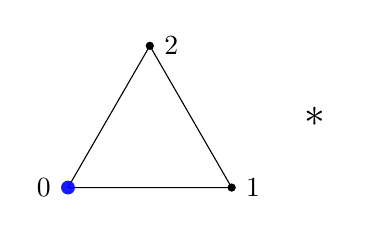
\begin{tikzpicture}[scale=.6]
\coordinate (A) at (210:2);
\coordinate (B) at (-30:2);
\coordinate (C) at (90:2);

\draw[draw=black] (A) -- (B) -- (C) -- (A);

\node[circle,fill=blue, opacity=.9, inner sep=0pt,minimum size=5pt, label=left:{0}] (a) at (A) {};
\node[circle,fill=black,inner sep=0pt,minimum size=3pt, label=right:{$1$}] (a) at (B) {};
\node[circle,fill=black,inner sep=0pt,minimum size=3pt, label=right:{$2$}] (a) at (C) {};

\node[scale=1.5] at (3.5,0.5) {$\ast$};
\end{tikzpicture}
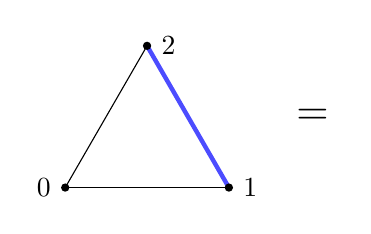
\begin{tikzpicture}[scale=.6]
\coordinate (A) at (210:2);
\coordinate (B) at (-30:2);
\coordinate (C) at (90:2);

\draw[draw=blue, ultra thick, draw opacity=.7] (B) -- (C);
\draw[draw=black] (C) -- (A);
\draw[draw=black] (A) -- (B);

\node[circle,fill=black,inner sep=0pt,minimum size=3pt, label=left:{$0$}] (a) at (A) {};
\node[circle,fill=black,inner sep=0pt,minimum size=3pt, label=right:{$1$}] (a) at (B) {};
\node[circle,fill=black,inner sep=0pt,minimum size=3pt, label=right:{$2$}] (a) at (C) {};

\node[scale=1.5] at (3.5,.5) {=};
\end{tikzpicture}
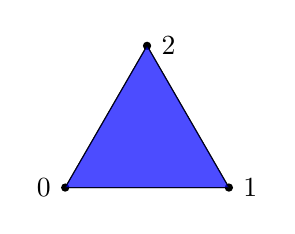
\begin{tikzpicture}[scale=.6]
\coordinate (A) at (210:2);
\coordinate (B) at (-30:2);
\coordinate (C) at (90:2);

\draw[draw=black] (A) -- (B) -- (C) -- (A);

\node[circle,fill=black,inner sep=0pt,minimum size=3pt, label=left:{$0$}] (a) at (A) {};
\node[circle,fill=black,inner sep=0pt,minimum size=3pt, label=right:{$1$}] (a) at (B) {};
\node[circle,fill=black,inner sep=0pt,minimum size=3pt, label=right:{$2$}] (a) at (C) {};

\draw[draw, fill=blue, opacity=.7] (A) -- (B) -- (C) -- (A);
\end{tikzpicture}
	\caption{Geometric representation of the join product of two basis elements. It depicts the identity $\pr \big( [0] \otimes [1,2] \big) = [0,1,2]$.}
	\label{f:join of faces}
\end{figure}
	% !TEX root = ../msimplicial.tex

\section{McClure-Smith and Barratt-Eccles  complexes } 
%We study an important example that will help us to understand how to prove our main 
%theorem.

In this section we introduce and compare a  multisimplicial and a simplicial  models of euclidean configuration spaces,
related respectively to the surjection operad by McClure-Smith and the Barratt-Eccles operad.

\begin{definition}
Let $Sur(k)$  be the $k$-fold multisimplicial set that has 
as $(i_1,\dots,i_k)$-multisimplexes
the surjective maps $$f:\{1,\dots,i_1+\dots+i_k+k\} \to  \{1,\dots,k\}$$ such that
the cardinality of $f^{-1}(l)$ is $i_l$, for $l=1,\dots,k$. We represent such maps by the sequence
$$f(1) \dots f(i_1+\dots+i_k+k)$$
The face map
$d^l_j$ removes the $(j+1)$-th occurrence of $l$ in a sequence, and the degeneracy map
$s^l_j$ doubles the $(j+1)$-th occurrence of $l$ in a sequence. 
So for example 
\begin{align*}d^2_0(12321)=1321 \\ d^2_1(12321)=1231 \\ s^1_0(121)=1121
\end{align*}
Degenerate multisimplices are exactly the sequences containing two equal adjacent terms.

The front  (resp. back) $(i_1,\dots,i_k)$-face of a sequence is the subsequence containing only the first (resp. last) 
$(i_l+1)$-values of $l$, for each
$l=1,\dots,k$.
\end{definition}


The (normalized) chain complexes 
of $Sur(k)$  $$\chi(k):=N(Sur(k))$$
were considered by McClure and Smith
\cite{MS},
who constructed an operad structure
on the collections of these complexes, the {\it surjection operad} $\chi$.


Also the geometric realizations 
$$\mathcal{F}(k)=\bars{Sur(k)}$$ appear in the work by McClure-Smith \cite{MS}, as explained in the appendix of \cite{Deligne}.   

The $k$-fold  $Sur(k)$ is filtered
by a nested family of $k$-fold multisimplicial sets
$$Sur_1(k) \subset Sur_2(k)  \subset \dots $$ such that $Sur(k) = {\rm colim}_n Sur_n(k)$. 

%A surjection belongs to $Sur_i(k)$
%if it does not contain an ordered %subsequence $ijij\dots$ with $i \neq j$ with more than $i+2$ values.

The collection of chain complexes 
$$\chi_n(k)=N(Sur_n(k))$$ 
gives a filtration of the surjection operad by suboperads

$$\chi_1 \subset \chi_2 \dots $$




%\begin{Remark}
%There is an interesting connection %between $Sur$ and t

We recall that the Barratt-Eccles simplicial sets $\mathcal{W}\Sigma_k$, where  $\Sigma_k$ is the symmetric group of permutations of $\{1,\dots,k\}$, is defined levelwise by
$\mathcal({W}\Sigma_k)_i=(\Sigma_k)^{i+1}$. The face $d_{j}$ removes the $(j+1)$-st permutation, and the degeneracy $s_j$ doubles the $(j+1)$-st permutation. There is an operad structure on the collection $W\Sigma_k$.
The (normalized) chain complex of $\mathcal{W}\Sigma_k$ is the Barratt-Eccles chain complex $$BE(k):=N(\mathcal{W}\Sigma_k)$$
and these complexes form an operad.
Berger and Fresse construct in \cite{BFsmall} 
  an operad map $TR:BE \to \chi$
and a collection of
chain maps $TC(k):\chi(k) \to BE(k)$
that are right inverses of $TR(k)$ and do not form an operad map.

We claim that $TC$ is induced by a map of simplicial sets
$$tc: Sur(k)^D \to \mathcal{W}\Sigma_k$$ that we define. 
\begin{definition}
Let $s$ be an $i$-simplex  of the diagonal $Sur(k)^D$, i.e. a sequence containing any value in $\{1,\dots,k\}$ exactly $i+1$ times. 
Then $tc(s):=(\sigma_0,\dots,\sigma_i)$ is a sequence of permutations where each $\sigma_j$ is the subsequence of $s$ containing the $(j+1)$-st occurrence of each value in $\{1,\dots,k\}$.
 \end{definition}

 For example 
 $$tc(122333112)=(123,231,312)$$

\begin{proposition} 
The homomorphism $TC$ by Berger-Fresse satisfies
$$TC=N(tc) \circ \ez$$ where
$$\ez: \chi(k) = N(Sur(k)) \to N(Sur(k)^D)$$ and $$N(tc):N(Sur(k)^D) \to N(\mathcal{W}\Sigma_k)=BE(k)$$
\end{proposition}

\begin{proof}
By inspection of the definition in \cite{BFsmall}. %more? signs? which convention?
\end{proof}

Also $\mathcal{W}$ is filtered \cite{BFsmall}, i.e.
there is a family of nested simplicial sets $$\mathcal{W}_1\Sigma_k \subset \mathcal{W}_2 \Sigma_k
 \subset \dots $$ such that 
$\mathcal{W}\Sigma_k={\rm colim}_d \mathcal{W}_d\Sigma_k$, that form a filtration by operads 
$$\mathcal{W}_1 subset \mathcal{W}_2 \subset \dots \mathcal{W}$$


The normalized chain functor defines 
$$BE_d(k):=N(\mathcal{W}_d \Sigma_k)$$ so that the operads $BE_d$  
form a filtration of $BE$.

%We observe that the simplicial map %$tc$ respects the filtration, sending 
%$\mathcal{W}_d\Sigma_k$ to %$Sur_d(k)^D$. 

%inserire mini-dimostrazione della filtrazione su grafi completi



%The geometric realizations satisfy 
%$$|Sur_d(k)| \simeq |\mathcal{W}_d\Sigma_k| \simeq F_k(\R^{d})$$
%where $F_k(\R^{d})$ is the ordered configuration space of $k$-tuples of points in  $\R^{d}$. 
We stress that the number of generators in $\chi_d(k)$, corresponding to non-degenerate surjections,
is much smaller than the corresponding number of generators in $BE_d(k)$. 
Let us consider the generating polynomial functions counting the generators
$$PB_d^k(x) = \sum_i rank(BE_d(k)_i) x^i $$ $$P\chi_d^k(x)=
\sum_i rank(\chi_d(k)_i) x^i$$   
Then for example 
\begin{align*}
& PB_2^4(x)=24(1+23x+104x^2+196x^3+184x^4+86x^5+16x^6)\\
& P\chi_2^4(x)=24(1+6x+10x^2+5x^3) \\
& \\
& PB_3^3(x) = 6(1+5x+25x^2+60x^3+70x^4+38x^5+8x^6 ) \\
&  P\chi_3^3(x)= 6(1+3x+7x^2+9x^3+6x^4+x^5)
\end{align*} 
Therefore the multisimplicial approach using $\chi$ is much more efficient than the simplicial
approach using $BE$, when performing computations as in \cite{formality}. 


%part by Andrea

	Both $\mathcal{W}$ and $Sur$ are filtered, i.e.
	there is a family of nested simplicial sets $$\mathcal{W}_1\Sigma_k \subset \mathcal{W}_2 \Sigma_k
	\subset \mathcal{W}_3 \Sigma_k
	\subset \dots $$ such that 
	$\mathcal{W}\Sigma_k={\rm colim}_d \mathcal{W}_d\Sigma_k$, and a family of nested $k$-fold simplicial sets
	$$Sur_1(k) \subset Sur_2(k)  \subset Sur_3(k)  \subset\dots $$ such that $Sur(k) = {\rm colim}_d Sur_d(k)$.
	
	\begin{remark}[Complete graphs]
		A complete graph is a weighted graph where for any couple of vertices (unordered) exists a unique edge of specified orientation.  For example:
\begin{equation*}
	\begin{tikzcd}
		\ & 2 & \  \\
		1 \arrow[ur,"2"] \arrow[rr] \arrow[dr,"3"']& \arrow[r,"1"] \arrow[u,"2"] & 3 \arrow[ul,"1"']  \\
		\ & 4 \arrow[ur,"4"'] \arrow[uu] & \
	\end{tikzcd}
\end{equation*}
Denote the set of complete graphs with $k$ vertices as $\mathcal{CG}(k)$.
Elements of $\mathcal{CG}(k)$ are representable as a pair $(\mu,\sigma)$, where $\mu$ is a collection of non-negative integers $\mu_{ij}\in\mathbb{N}$, $i,j\in \left\lbrace 1,\dots, k \right\rbrace $
% associeted to the correspondent pair of vertices,
  and $\sigma$ is a permutation in $\Sigma_{k}$ giving orientation of edges as the order of appearance of $i$ and $j$ in that permutation.
%   $\sigma=(\sigma(1)\sigma(2)\dots \sigma(k))$, the 'arrow' goes from the first appearing, to the second. It is easier if we define the permutation $\sigma_{ij}$ obtained omitting all occurrences of number different from $i$ and $j$ in the permutation, and then see the order. This notation is useful in what will follow.
For example the permutation correspondent to the figure is $(1432)$ .
$\sigma_{ij}$ will denote the permutation obtained omitting all elements different from $i$ and $j$.
	\end{remark}

\begin{remark}[Complete graphs form a poset]
	$\mathcal{CG}(k)$ has a poset structure as follow: 
	\begin{equation*}
		(\mu,\sigma)\le (\nu,\tau) \ \ \text{ if and only if } \ \ (\mu_{ij}<\nu_{ij}) \ \ \text{ or } \ \ (\mu_{ij},\sigma_{ij})= (\nu_{ij},\tau_{ij}) 
	\end{equation*}
	for each pair $\left\lbrace i,j\right\rbrace \subset\left\lbrace 1,\dots,k  \right\rbrace $.
\end{remark}	

%In both cases of multisimplicial set $Sur$ and simplicial set of Barratt-Eccles (We can call them just $X$ for now) we need to give a way to find certain subsets of elements using complete graphs. In particular we want to define what means to belong to the subset $X_{(\mu,\sigma)}\subseteq X$ and then define 
%\begin{equation}
%	\label{def}
%	X_{n}=\bigsqcup_{\mu_{ij}\le n} X_{(\mu,\sigma)}
%\end{equation}

	\begin{definition}[Filtration of the surjection multisimplicial set $Sur$]
		Fix a surjection $f\in Sur(k)_{i_{1},\dots,i_{k}}$. For any pair $(i,j)$ with $i< j$, $f_{ij}$ is the subsequence of $f(1) \dots f(i_1+\dots+i_k+k)$ obtained omitting all the occurrences of elements different from $i$ and $j$. 
%		For example, let $31231 \in Sur(3)_{2,1,2}$, we have $(31231)_{12}=121$, $(31231)_{23}=323$ and $(31231)_{13}=3131$.
		The surjection $f$ belongs to $Sur_{(\mu,\sigma)}(k)\subseteq Sur(k)$ if for all pairs $(i,j)$, $i< j$ either the sequence $f_{ij}$ has strictly less than $\mu_{ij}$ variation number
%		, that is the amount of times that the order of $i$ and $j$ change ,
		 or the sequence $f_{ij}$ has exactly $\mu_{ij}$ as variation number and the permutation formed by the first occurences of $i$ and $j$ in $f_{ij}$ agrees with $\sigma_{ij}$. Accordingly to this $f$ belongs to $Sur_{n}(k)\subseteq Sur(k)$ if and only if for all pairs $(i,j)$, $i< j$ the sequence $f_{ij}$ has strictly less than $n$ variation number. This means:
		 \begin{equation*}
		 	\label{def}
		 	Sur_{n}(k)=\bigsqcup_{\mu_{ij}< n} Sur_{(\mu,\sigma)}(k)
		 \end{equation*}
%		\\
%		\\
%		Returning to the example above we have $\mu_{12}(31231)=1$, $\mu_{23}(31231)=1$ and $\mu_{13}(31231)=2$ so that $31231\in Sur_{(\mu,\sigma)}(3)_{2,1,2}$  
%		\begin{itemize}
%		\item if $\mu_{12}>1$, $\mu_{23}>1$ and $\mu_{13}>2$ and any $\sigma\in \Sigma_{3}$;
%		\item if some $\mu_{ij}=\mu(f)_{ij}$ and the first occurences of $i$ and $j$ in $f_{ij}$ agrees with $\sigma_{ij}$.
%		\end{itemize}
%	    In our example we obtain that, by equation \ref{def},
%	    $31231\in Sur_{3}(k)_{2,1,2}$
%	    \\
%	    \\
	    We have obtained the filtration $$Sur_1(k) \subset Sur_2(k)  \subset Sur_3(k)  \subset \dots $$
	    that induces the filtration of the correspondent diagonal simplicial set 
	    $$Sur_1(k)^{D} \subset Sur_2(k)^{D}  \subset Sur_3(k)^{D}  \subset\dots $$
	    
	\end{definition}

	\begin{definition}[Filtration of the Barratt-Eccles simplicial set $\mathcal{W}\Sigma_k$]
	Fix an element  $w\in (\mathcal{W}\Sigma_k)_{d}$, $w=(w_{1},\dots , w_{d})$ with $w_{h}\in \Sigma_k$. For any pair $(i,j)$ with $i< j$, denote $w_{ij}=(w_{1,ij},\dots , w_{d,ij})$ where $w_{h,ij}$ is the subsequence of $w_{h}$ obtained omitting all the occurrences of elements different from $i$ and $j$. 
%	For example, let $(123,231,312) \in (\mathcal{W}\Sigma_3)_{3}$, we have $(123,231,312)_{12}=(12,21,12)$, $(123,231,312)_{23}=(23,23,32)$ and $(123,231,312)_{13}=(13,31,31 )$.
	The element $w$ belongs to $\mathcal{W}_{(\mu,\sigma)}\Sigma_k\subseteq \mathcal{W}\Sigma_k$ if for all pairs $(i,j)$, $i< j$ either the sequence $f_{ij}$ has strictly less than $\mu_{ij}$ variation number
%	, that is, as before,  the amount of times that the order of $i$ and $j$ change ,
	 or the sequence $w_{ij}$ has exactly $\mu_{ij}$ as variation number with the first permutation equal to $\sigma_{ij}$. Accordingly to this $w$ belongs to $\mathcal{W}_{n}\Sigma_k\subseteq \mathcal{W}\Sigma_k$ if and only if for all pairs $(i,j)$, $i< j$ the sequence $w_{ij}$ has strictly less than $n$ variation number. This means:
	  \begin{equation*}
	 	\label{def}
	 	\mathcal{W}_{n}\Sigma_k=\bigsqcup_{\mu_{ij}< n} \mathcal{W}_{(\mu,\sigma)}\Sigma_{k}
	 \end{equation*}
	\\
	\\
%	Returning to the example above we have $\mu_{12}(123,231,312)=2$, $\mu_{23}(123,231,312)=1$ and $\mu_{13}(123,231,312)=1$ so that $(123,231,312)\in (\mathcal{W}_{(\mu,\sigma)}\Sigma_3)_{3}$
%	\begin{itemize}
%		\item if $\mu_{12}>2$, $\mu_{23}>1$ and $\mu_{13}>1$ and any $\sigma\in \Sigma_{3}$;
%		\item if some $\mu_{ij}=\mu_{ij}(w)$ and the first permutation of $w$ is equal to $\sigma_{ij}$.
%	\end{itemize}
%	In our example we obtain that, by equation \ref{def},
%	$(123,231,312)\in (\mathcal{W}_{3}\Sigma_3)_{3}$
%	\\
%	\\
	We have obtained the filtration $$\mathcal{W}_1\Sigma_k \subset \mathcal{W}_2 \Sigma_k
	\subset \mathcal{W}_3 \Sigma_k
	\subset \dots $$ 
%	that is the other one we need in $tc$ definition.
	
\end{definition}
 
% In both cases, to see even the role of permutations we'll use always pairs $(\mu,\sigma)$ with $\mu$ exactly the collection of variation numbers obtained from the initial element so that the permutation is uniquely determined, and $(\mu,\sigma)$ is minimal in the poset.
% \\
% In our examples 
% \begin{itemize}
% 	\item $31231\in Sur_{(\mu,\sigma)}(3)_{2,1,2} \subseteq Sur_{3}(3)_{2,1,2}$ with $(\mu_{12},\mu_{13},\mu_{23})=(1,2,1)$ and $\sigma=(312)$
% 	\item $(123,231,312)\in (\mathcal{W}_{(\mu,\sigma)}\Sigma_3)_{3} \subset (\mathcal{W}_{3}\Sigma_3)_{3}$ with $(\mu_{12},\mu_{13},\mu_{23})=(2,1,1)$ and $\sigma=(123)$
% \end{itemize}
%	We observe that the simplicial map $tc$ respects the filtration, sending 
%	$Sur_d(k)^D$ to $\mathcal{W}_d\Sigma_k$ 
%	\\
%	\begin{example}
%	We are givine some example of the compatibility of $tc$ to visualize why it works in general.
%	Let $122333112 \in Sur(3)^{D} $
%	\begin{itemize}
%		\item $(122333112)_{12}=122112\rightarrow \mu_{12}=2$
%		\item $(122333112)_{13}=133311\rightarrow \mu_{13}=1$
%		\item $(122333112)_{23}=223332\rightarrow \mu_{23}=1$
%	\end{itemize}
%So $\mu=(\mu_{12},\mu_{13},\mu_{23})=(2,1,1)$
%and the first occurrences of $1,2,3$ give us the permutation $\sigma=(123)$ $\Rightarrow$ $122333112 \in Sur_{((2,1,1),(123))}(3)^{D}$ $\Rightarrow$ $122333112 \in Sur_{3}(3)^{D}$.
%Now applying $tc$ we obtain $tc(122333112)=(123,231,312)\in (\mathcal{W}\Sigma_3)_{3} $
%\begin{itemize}
%\item $(123,231,312)_{12}=(12,21,12)\rightarrow \mu_{12}=2$
%\item $(123,231,312)_{13}=(13,31,31)\rightarrow \mu_{13}=1$
%\item $(123,231,312)_{23}=(23,23,32)\rightarrow \mu_{23}=1$
%\end{itemize}
%So $\mu=(\mu_{12},\mu_{13},\mu_{23})=(2,1,1)$
%and the first permutation in $(123,231,312)$ give us the permutation $\sigma=(123)$ $\Rightarrow$ $(123,231,312) \in (\mathcal{W}_{((2,1,1),(123))}\Sigma_{3})_{3}$ $\Rightarrow$ $(123,231,312) \in (\mathcal{W}_{3}\Sigma_{3})_{3}$.
%
%
%
%	\end{example}

\begin{lemma}[Compatibility of $tc$]
	We have that the map $tc:Sur(k)^{D}\rightarrow \mathcal{W}\Sigma_{k}$ is compatible with the filtrations, in the sense that 
	$$tc(Sur_{n}(k)^{D})\subseteq \mathcal{W}_{n}\Sigma_{k}$$
	
	In particular 
	$$tc(Sur_{(\mu,\sigma)}(k)^{D})\subseteq \mathcal{W}_{(\mu,\sigma)}\Sigma_{k}$$
\end{lemma}
\begin{proof}
Let  $f\in Sur_{n}(k)^{D}$ be an $m$-simplex and denote 
%This means $f$ is a sequence  $f(1)f(2)\dots f(km+m)$ containing any value in $\left\lbrace 1,\dots,k\right\rbrace $ exactly $m+1$ times and so 
$tc(f)=w=(w_{1},\dots,w_{m+1})\in (\mathcal{W}\Sigma_{k})_{m+1}$. We suppose the variation numbers of $f$ are $\mu_{ij}$, and claim that $w$ has no more than these as variation numbers.  Let us denote variation numbers of $w$ as $\mu_{ij}'$. 
Let us consider just the subsequence of including only indices $(i,j)$, $f_{ij}$. If $f^{-1}(i)=\left\lbrace i_{1}<i_{2}<\dots<i_{m+1}\right\rbrace $ and $f^{-1}(j)=\left\lbrace j_{1}<j_{2}<\dots<j_{m+1}\right\rbrace $ then $f^{-1}(i)\cap f^{-1}(j)=\emptyset$ and we can express the above mentioned subsequence as follow:
\begin{equation*}
\begin{split}
f_{ij}=&f(i_{1})f(i_{2})\dots f(i_{k})f(j_{1})\dots f(j_{l})f(i_{k+1})\dots f(i_{k+t})f(j_{l+1})\dots f(j_{l+s})\dots \dots \dots  \\
&\dots \dots \dots  f(j_{h})\dots f(j_{m+1})f(i_{r})\dots f(j_{m+1})
\end{split}
\end{equation*}
We are assuming $i$ appears first, so the starting order of $f_{ij}$ and $w_{ij}$ is $(i,j)$ (the argument is indipendent of this choice and it is in fact the same in the inverse case).
%We can arrange the sequence $f_{ij}$ in a table 
%\begin{equation*}
%\left|  \ \ \ \begin{split}
%	&f(i_{1})\dots f(i_{k})\\
%	&f(j_{1})\dots f(j_{l}) \\
%	&f(i_{k+1})\dots f(i_{k+t}) \\
%	&f(j_{l+1})\dots f(j_{l+s}) \\
%	&\dots \dots \dots  \\
%	&f(j_{h})\dots f(j_{m+1})\\
%	&f(i_{r})\dots f(j_{m+1})
%\end{split}
%\right. 
%\end{equation*}
%and the variation number associeted $\mu_{ij}$ will be the number of lines minus $1$. This because we're starting with a specific order of indices (in this case $(i,j)$)  and we count $+1$ every time the index change from this moment. 



We arrange the sequence in a table as follow: (it is important to note that columns of this table will be exactly elements $(w_{1},\dots, w_{m+1})$)
\begin{enumerate}
	\item [-] Write the first subsequences of $i$ and $j$ as first and second row of the table;
\begin{equation*}
\begin{split}
		&f(i_{1})\dots f(i_{k}) \\
		&f(j_{1})\dots f(j_{l}) \\
	\end{split}
\end{equation*}
	\item If the second row is longer (not equal), then write the following subsequence (of the appearing index) starting from under the element $f(j_{\_+1})$ or $f(i_{\_+1})$
\begin{equation*}
	\begin{split}
		&f(i_{1})\dots f(i_{k}) \ \ \ \ \ \ \ \ \ \ \ \ \ \ \ \ \ \ \ \ \ \ \ \ \ \ \ \ \ \ \ \ \ \ \ \ \ \ \ \ \ \ \ \ \ \ \ \ \ \ \ \ \ \ \  \mu_{ij}=\mu_{ij}+1\\
		&f(j_{1})\dots f(j_{k})f(j_{k+1})\dots f(j_{l})\ \ \ \ \ \ \ \ \ \ \ \ \ \ \ \ \ \ \ \ \ \ \ \ \ \ \ \ \ \ \ \ \ \ \ \mu_{ij}'=\mu_{ij}'+1 \\
		& \ \ \ \ \ \ \ \ \ \ \ \ \ \ \ \ \ \ f(i_{k+1})\dots f(i_{k+t})
	\end{split}
\end{equation*}
%Because adding a line here means we have a change of order in $tc(f)_{ij}$ the variation number increase by one.
\item If the second row is shorter equal, then write the following subsequence (of the appearing index) continuing from the correspondent element $f(i_{\_})$ or $f(j_{\_})$
\begin{equation*}
	\begin{split}
		&f(i_{1})\dots f(i_{l})f(i_{l+1})f(i_{k})f(i_{k+1})\dots f(i_{k+t}) \ \ \ \ \ \ \ \ \ \ \ \ \ \ \ \ \ \mu_{ij}=\mu_{ij}+1\\
		&f(j_{1})\dots f(j_{l}) \ \ \ \ \ \ \ \ \ \ \ \ \ \ \ \ \ \ \ \ \ \ \ \ \ \ \ \ \ \ \ \ \ \ \ \ \ \ \ \ \ \ \ \ \ \ \ \ \ \ \ \ \ \ \  \mu_{ij}'=\mu_{ij}'\\
	\end{split}
\end{equation*}
%Because the number of lines does not change we haven't a change of order and so the variation number do not increase.
\item [-] If we consider now the last two rows of the table obtained as a new first and second, we can continue studying cases $1$ and $2$, obtaining a finite algorithm.
\end{enumerate}
We finally obtain $\mu_{ij}'\le \mu_{ij}$.\\
Moreover $tc$ respects permutations, because if we have certain variation numbers associated to $f$, we can associate a specific permutation formed by the first occurreces of each value in $\left\lbrace 1,\dots, k \right\rbrace $, that is exactly $w_{1}$.
Both assertions follow.
\end{proof}

\begin{corollary}
	The map $tc_{n}:Sur_{n}(k)^{D}\rightarrow \mathcal{W}_{n}\Sigma_{k}$ is a weak equivalence.
\end{corollary}

\begin{proof}
	Follow from the commutative diagram below build up with all weak equivalences
	\begin{equation*}
		\begin{tikzcd}
			colim_{(\mu,\sigma)}Sur_{(\mu,\sigma)}(k)^{D} \arrow[r,"tc_{(\mu,\sigma)}"] \arrow[d]& colim_{(\mu,\sigma)}\mathcal{W}_{(\mu,\sigma)}\Sigma_{k} \arrow[d] \\
			Sur_{n}(k)^{D}\arrow[r] & \mathcal{W}_{n}\Sigma_{k}& 
		\end{tikzcd}
	\end{equation*}
\end{proof}

Let  $F_k(\R^{d})$ be the ordered configuration space of $k$-tuples of points in  $\R^{d}$. 

\begin{proposition}
The geometric realizations satisfy 
$$|Sur_d(k)| \simeq |W_d(k)|  \simeq F_k(\R^{d})$$
\end{proposition}

\begin{proof}
The configuration space is a homotopy colimit of contractible spaces along the same poset.
\end{proof}
%	
\section{\pdfEinfty-structures} \label{s:operads and props}

The goal of this section is to define an explicit $E_\infty$-algebra structure on multisimplicial cochains.
That is to say, a product descending to the ring structure on cohomology together with a coherent family of homotopies correcting its lack of commutativity at the cochain level.

We begin by reviewing basic material concerning the theory of operads and props, referring the reader to, for example, \cite{markl2008props} for a more complete treatment.
We then recall the definition of the finitely presented prop $\M$ introduced in \cite{medina2020prop1} and whose associated operad is a model for the $E_\infty$-operad.
Given its small number of generators and relations, $\M$ is well suited to define $E_\infty$-structures.
We recall from the same source one such structure on simplicial cochains, which we monoidally extend to achieve our stated goal.

\subsection{Symmetric modules and bimodules}

Let $\S$ be the category whose objects are the natural numbers and whose set of morphisms between $m$ and $n$ is empty if $m \neq n$ and is otherwise the symmetric group $\S_n$.
A \textit{left $\S$-module} (resp. \textit{right} $\S$-\textit{module} or $\S$-\textit{bimodule}) is a functor from $\S$ (resp. $\S^\op$ or $\S \times \S^\op$) to $\Ch$.
In this paper we prioritize left module structures over their right counterparts.
As usual, taking inverses makes both perspectives equivalent.
We respectively denote by $\Smod$ and $\Sbimod$ the categories of left $\S$-modules and of $\S$-bimodules with morphisms given by natural transformations.

The group homomorphisms $\S_n \to \S_n \times \S_1$ induce a forgetful functor
\[
\forget \colon \Sbimod \to \Smod,
\]
given explicitly by $\forget(\cP)(r) = \cP(1, r)$ for $r \in \N$.
The similarly defined forgetful functor to right $\S$-modules will not be used.

\subsection{Composition structures}

We can define \textit{operads} and \textit{props} by enriching $\S$-modules and $\S$-bimodules with certain composition structures.
For a complete presentation of these concepts we refer to Definition~11 and 54 of \cite{markl2008props}.
Intuitively, using examples defined in the next subsection, operads and props can be understood by abstracting the composition structure naturally present in the left $\S$-module $\End^C$ (or right $\S$-module $\End_C$), naturally an operad, and the $\S$-bimodule $\End^C_C$, naturally a prop.
We remark that the prop structure on $\cP$ restricts to an operad structure on $\forget(\cP)$.

\subsection{Representations}

Given a chain complex $C$ define
\begin{gather*}
\End^C(r) = \Hom(C, C^{\otimes r}), \qquad
\End_C(r) = \Hom(C^{\otimes r}, C), \\
\End^C_C(r, s) = \Hom(C^{\otimes r}, C^{\otimes s}),
\end{gather*}
with their natural operad and prop structures respectively.
We remark that the forgetful functor $\forget$ sends $\End^C_C$ to $\End^C$.

Let $C$ be a chain complex, $\cO$ an operad, and $\cP$ a prop.
An $\cO$-\textit{coalgebra} (resp. $\cO$-\textit{algebra} or $\cP$-\textit{bialgebra}) structure on $C$ is a structure preserving morphism $\cO \to \End^C$ (resp. $\cO \to \End_C$ or $\cP \to \End_C^C$).

\subsection{\pdfEinfty-operads}

Recall that a \textit{free $\S_r$-resolution} of a chain complex $C$ is a quasi-isomorphism $R \to C$ from a chain complex of free $\k[\S_r]$-modules.

An $\S$-module $M$ is said to be $E_{\infty}$ if there exists a morphism of $\S$-modules $M \to \underline{\k}$ inducing for each $r \in \N$ a free $\S_r$-resolution $M(r) \to \k$.

An operad is said to be $E_{\infty}$ if its underlying $\S$-module is $E_\infty$.

\subsection{Free prop construction} \label{ss:free prop}

\begin{figure}
	\boxed{\begin{tikzpicture}[scale=.6]
\draw (1,3.7) to (1,3); 

\draw (1,3) to [out=205, in=90] (0,0);

\draw [shorten >= 0cm] (.6,2.73) to [out=-100, in=90] (2,0);

\draw [shorten >= .15cm] (1,3) to [out=-25, in=30, distance=1.1cm] (1,1.5);
\draw [shorten <= .1cm] (1,1.5) to [out=210, in=20] (0,1);

\node at (1,3.9){};
\node at (0,-.32){};
\node at (2,-.32){};

\node at (3,1.5){$\sim$\ \ \ };
\end{tikzpicture}
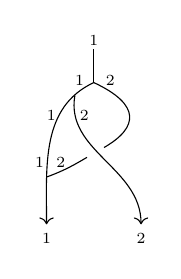
\begin{tikzpicture}[scale=.6]
\draw (1,3.7) to (1,3); 

\draw [->](1,3) to [out=205, in=90] (0,0);

\draw [shorten >= 0cm,->] (.6,2.73) to [out=-100, in=90] (2,0);

\draw [shorten >= .15cm] (1,3) to [out=-25, in=30, distance=1.1cm] (1,1.5);
\draw [shorten <= .1cm] (1,1.5) to [out=210, in=20] (0,1);


\def\x{.8}

\node[scale=\x] at (1,3.9){$\scriptstyle 1$};

\node[scale=\x] at (.7,3.05){$\scriptstyle 1$};
\node[scale=\x] at (1.35,3.05){$\scriptstyle 2$};

\node[scale=\x] at (.1,2.3){$\scriptstyle 1$};
\node[scale=\x] at (.8,2.3){$\scriptstyle 2$};

\node[scale=\x] at (-.15,1.3){$\scriptstyle 1$};
\node[scale=\x] at (.3,1.3){$\scriptstyle 2$};

\node[scale=\x] at (0,-.3){$\scriptstyle 1$};
\node[scale=\x] at (2,-.3){$\scriptstyle 2$};
\end{tikzpicture}}
	\caption{Immersed graphs represent labeled directed graphs with the direction implicitly given from top to bottom and the labeling from left to right.}
	\label{f:immersion}
\end{figure}

The \textit{free prop} $\free(M)$ generated by an $\S$-bimodule $M$ is constructed using isomorphism classes of directed graphs with no directed loops that are enriched with the following labeling structure.
We think of each directed edge as built from two compatibly directed half-edges.
For each vertex $v$ of a directed graph $\Gamma$, we have the sets $in(v)$ and $out(v)$ of half-edges that are respectively incoming to and outgoing from $v$.
Half-edges that do not belong to $in(v)$ or $out(v)$ for any $v$ are divided into the disjoint sets $in(\Gamma)$ and $out(\Gamma)$ of incoming and outgoing external half-edges.
For any positive integer $n$ let $\overline{n} = \{1, \dots, n\}$ and set $\overline{0} = \emptyset$.
For any finite set $S$, denote the cardinality of $S$ by $|S|$.
The labeling is given by bijections
\[
\overline{|in(\Gamma)|}\to in(\Gamma), \qquad
\overline{|out(\Gamma)|}\to out(\Gamma),
\]
and
\[
\overline{|in(v)|}\to in(v), \qquad
\overline{|out(v)|}\to out(v),
\]
for every vertex $v$.
We refer to the isomorphism classes of such labeled directed graphs with no directed loops as $(n,m)$\textit{-graphs} denoting the set of these by $\graphs(m,n)$.
We use graphs immersed in the plane to represent elements in $\graphs(m,n)$, please see \cref{f:immersion}.
We consider the right action of $\S_n$ and the left action of $\S_m$ on a $(n,m)$-graph given respectively by permuting the labels of $in(\Gamma)$ and $out(\Gamma)$.
This action defines the $\S$-bimodule structure on the free prop
\begin{equation} \label{e:free prop}
\free(M)(m,n) \ = \bigoplus_{\Gamma \in \graphs(m,n)} \bigotimes_{v \in Vert(\Gamma)} out(v) \otimes_{\S_q} M(p, q) \otimes_{\S_p} in(v),
\end{equation}
where we simplified the notation writing $p$ and $q$ for $\overline{|in(v)|}$ and $\overline{|out(v)|}$ respectively.
The composition structure is defined by (relabeled) grafting and disjoint union.

\subsection{The prop $\M$}

We now recall the model of $E_\infty$ that is central to our constructions.

\begin{definition}
	Let $\M$ be the prop generated by
	\begin{equation} \label{e:generators of M}
	\counit\,, \hspace*{.6cm} \coproduct\,, \hspace*{.6cm} \product,
	\end{equation}
	in degrees $0$, $0$ and $1$ respectively, and boundaries
	\begin{equation} \label{e:boundary of M}
	\partial\ \counit = 0,
	\hspace*{.6cm}
	\partial\, \coproduct = 0,
	\hspace*{.6cm}
	\partial \product = \ \boundary\,,
	\end{equation}
	modulo the prop ideal generated by
	\begin{equation} \label{e:relations of M}
	\leftcounitality\,, \hspace*{.6cm} \rightcounitality\,, \hspace*{.6cm} \productcounit.
	\end{equation}
\end{definition}

Explicitly, any element in $\M(m,n)$ can be written as a linear combination of the $(m,n)$-graphs generated by those in \eqref{e:generators of M} via grafting, disjoint union and relabeling, modulo the prop ideal generated by the relations in \eqref{e:relations of M}. Its boundary is determined, using \eqref{e:free prop}, by \eqref{e:boundary of M}.

As proven in \cite[Theorem 3.3]{medina2020prop1} we have the following.

\begin{proposition}
	The operad $\UM$ is $E_{\infty}$.
\end{proposition}

We remark that, as proven in \cite{medina2018prop2}, this prop is obtained from applying the functor of cellular chains to a finitely presented prop over the category of CW-complexes.

\subsection{Hopf operads and props}

So far we have consider operad and props over the category $\Ch$ but, since $\coAlg$ is also a symmetric monoidal category, we can consider them over $\coAlg$.
That is to say, demand that all defining chain complexes be coalgebras and all compositions be morphisms of these.
We refer to operads and props over $\coAlg$ as \textit{Hopf operads} and \textit{props} respectively.

If $\cO$ is a Hopf operad, the category $\coAlg_\cO$ is monoidal.
The structure maps of a product of $\cO$-coalgebras $C \otimes C^\prime$ are given by
\[
\begin{tikzcd} [column sep = normal, row sep=normal]
\cO(r) \otimes (C \otimes C^\prime) \arrow[r, "\Delta_\cO \otimes \id"] &[10 pt]
\cO(r) \otimes \cO(r) \otimes (C \otimes C^\prime) \arrow[d, "Sh"'] & \\ &
\big(\cO(r) \otimes C \big) \otimes \big( \cO(r) \otimes C \big) \arrow[r] &
C^{\otimes r} \otimes C^{\prime\, \otimes r} \arrow[d, "Sh"] & \\ & &
(C \otimes C^\prime)^{\otimes r}.
\end{tikzcd}
\]
Similarly, if $\cP$ is a Hopf prop then its category of representations is also monoidal.

\subsection{Hopf structure on $\M$} \label{ss:hopf prop M}

As proven in \cite{medina2021cobar}, the prop $\M$ is Hopf with coproduct $\Delta_\M$ and counit $\varepsilon_\M$ induced by
\begin{align*}
\coproduct & \mapsto \coproduct \otimes \coproduct \,, &
\coproduct & \mapsto 1, \\
\counit \ & \mapsto \ \counit \ \otimes \ \counit \,, &
\counit \ & \mapsto 1, \\
\product & \mapsto \rightboundary \ \otimes \product + \product \otimes \ \leftboundary \,, &
\coproduct & \mapsto 0.
\end{align*}
It follows from the previous subsection that $\coAlg_\UM$ is a monoidal category.

\subsection{Simplicial $E_{\infty}$-structure} \label{ss:e-infty on simplicial}

We review from \cite{medina2020prop1} a natural $\mathcal M$-structure on the chains of standard simplices.
These define, for any simplicial set, a natural $\UM$-structure on its chains generalizing the $E_{\infty}$-coalgebra structures constructed by McClure--Smith \cite{mcclure2003multivariable} and Berger--Fresse \cite{berger2004combinatorial}.

An $\M$-structure is specified by three linear maps, the images of the generators
\[
\counit, \quad \coproduct, \quad \product,
\]
satisfying the relations in the presentation of $\mathcal M$.
For the chains on standard simplices, the first two generators are send respectively to the counit and coproduct of the Alexander--Whitney coalgebra, and the third generator to an algebraic version of the join $\ast \colon \chains(\simplex^n)^{\otimes 2} \to \chains(\simplex^n)$ defined by
\[
\left[v_0, \dots, v_p \right] \ast \left[v_{p+1}, \dots, v_q\right] = \begin{cases} (-1)^{p+|\pi|} \left[ v_{\pi(0)}, \dots, v_{\pi(q)} \right] & \text{ if } v_i \neq v_j \text{ for } i \neq j, \\
0 & \text{ otherwise}, \end{cases}
\]
where $\pi$ is the permutation that orders the set of vertices, and $(-1)^{|\pi|}$ is its sign.

From \cite{medina2020prop1} we have the following result.

\begin{proposition} \label{p:simplicial chain bialgebra}
	For every $n \in \mathbb{N}$, the assignment
	\[
	\counit \mapsto \epsilon, \quad \coproduct \mapsto \Delta, \quad \product \mapsto \ast,
	\]
	defines a natural $\mathcal M$-structure on $\chains(\simplex^n)$.
\end{proposition}

The chains on general simplicial sets are not equipped with an $\M$-structure, but using the forgetful functor from $\biAlg_{\M}$ to the cocomplete category $\coAlg_\UM$ allows us to Yoneda extend the induced natural $\UM$-structures on standard simplices to all simplicial sets.
Specifically, we obtain an extension of the Alexander--Whitney coalgebra in the form of a lift:
\[
\begin{tikzcd}[column sep=normal, row sep=small]
& \coAlg_\UM \arrow[d] \\
\sSet \arrow[r, "\schains"]
\arrow[ur, "\schainsUM", out=60, in=180, near start, dashed]
& \Ch.
\end{tikzcd}
\]

A similar argument using the duality functor provides simplicial cochains with a $\UM$-algebra structure.

\subsection{Multisimplicial \pdfEinfty-structure}

We use the monoidal structure on $\coAlg_\UM$ to define a lift of the functor of multisimplicial chains to the category of $\UM$-coalgebras
\[
\mchainskUM \defeq \Big(\schainsUM\Big)^{\otimes k}
\]
fitting in the following commutative diagram:
\[
\begin{tikzcd}[column sep=normal, row sep=small]
& \coAlg_\UM \arrow[d] \\
\arrow[ur, "\mchainskUM", out=60, in=180, near start, dashed]
\sSet^k \arrow[r, "\mchainsk"]
& \Ch.
\end{tikzcd}
\]

As before, a similar construction provides multisimplicial cochains with a $\UM$-algebra structure.

\subsection{Explicit description}

We now introduce linear maps on the chains of representable multisimplicial sets defining a natural $\M$-structure on each of them.
These forget to natural $\UM$-structures defining, via Yoneda extension, the functor $\mchainskUM$ from the previous subsection.
The case $k = 1$ reduces to the $\M$-structure on simplicial chains, which we monoidally extend for $k > 1$.

Let $C$ denote $\mchainsk(\simplex^{n_1} \times \dots \times \simplex^{n_k})$ and consider basis elements $x = x_1 \otimes \dots \otimes x_k$ and $y = y_1 \otimes \dots \otimes y_k$ in $C$.

The \textit{multisimplicial counit} $\varepsilon \colon C \to \k$ is defined by
\[
\varepsilon(x) = \varepsilon(x_1) \dotsm \varepsilon(x_k).
\]

The \textit{multisimplicial coproduct} $\Delta \colon C \to C \otimes C$ is defined by
\[
\Delta (x_1 \otimes \dots \otimes x_n) =
\sum \pm \left( x_1^{(1)} \otimes \dots \otimes x_n^{(1)} \right) \otimes
\left( x_1^{(2)} \otimes \dots \otimes x_n^{(2)} \right),
\]
where the sign is determined using the Koszul convention, and we are using Sweedler's notation
\[
\Delta(x_i) = \sum x_i^{(1)} \otimes x_i^{(2)}
\]
for the coproduct $\Delta \colon \chains(\simplex^{n_i}) \to \chains(\simplex^{n_i})^{\otimes 2}$.

The \textit{multisimplicial join} $\ast \colon C \otimes C \to C$ is defined by
\begin{align*}
(x_1 \otimes \dots \otimes x_n) \ast (y_1 \otimes \dots \otimes y_n) =
(-1)^{|x|} \sum_{i=1}^n x_{<i}\, \epsilon(y_{<i}) \otimes x_i \ast y_i \otimes \epsilon(x_{>i}) \, y_{>i},
\end{align*}
where
\begin{align*}
x_{<i} & = x_1 \otimes \dots \otimes x_{i-1}, &
y_{<i} & = y_1 \otimes \dots \otimes y_{i-1}, \\
x_{>i} & = x_{i+1} \otimes \dots \otimes x_n, &
y_{>i} & = y_{i+1} \otimes \dots \otimes y_n,
\end{align*}
with the convention
\[
x_{<1} = y_{<1} = x_{>n} = y_{>n} = 1 \in \Z,
\]
and $x_i \ast y_i$ is the join in $\chains(\simplex^{n_i})$.

\subsection{Steenrod operations}

Throughout this subsection let us consider $\k$ to be the finite field $\Fp$ and $X$ a multisimplicial set.

Since the complex of cochains on $X$ is an $E_\infty$-algebra, the mod $p$ cohomology $H_\bullet^{\vee}(X; \Fp)$ is a priori equipped with an action of the Steenrod algebra \cite{steenrod1962cohomology, may1970general}.
As an application of the explicit construction of a natural $\UM$-coalgebra structure on $\chains(X)$, we can describe at the cochain level this action using the constructions of \cite{medina2020maysteenrod}.
More explicitly, let $\Cp$ be the cyclic group of order $p$ and
\[
\begin{tikzcd} [column sep = .5cm]
\cW(p) = \Fp[\Cp]\{e_0\} & \arrow[l, "\,T"'] \Fp[\Cp]\{e_1\} & \arrow[l, "\,N"'] \Fp[\Cp]\{e_2\} & \arrow[l, "\,T"'] \dotsb
\end{tikzcd}
\]
be the minimal free resolution of $\Fp$ as an $\Fp[\Cp]$-module.
Consider the $\Cp$-equivariant quasi-isomorphism $\psi_\UM \colon \cW(p) \to \UM(p)$ constructed in \cite{medina2020maysteenrod}, and denote by $\psi^{\msimplex{k}}$ its composition with the morphism $\UM \to \End_{\chains(X)}$ defining our $\UM$-coalgebra structure on $\chains(X)$.

If $p$ is the even prime and $s$ is an integer, the \textit{Steenrod operation}
\begin{equation*}
P_s \colon H^\vee_\bullet(A; \bbF_2) \to H^\vee_{\bullet + s}(A; \bbF_2)
\end{equation*}
is defined by sending the class represented by a cocycle $\alpha \in \cochains(X; \bbF_2)$ of degree $q$ to the class represented by the cochain
\[
c \mapsto (\alpha \otimes \alpha) \, \psi^{\msimplex{k}}(e_{s-q})(c).
\]

We remark that \textit{Steenrod $(2,i)$-products}, usually referred to as cup-$i$ products, are given by
\begin{equation} \label{e:cup-i products}
(\alpha \smallsmile_i \beta)(c) = (\alpha \otimes \beta) \, \psi^{\msimplex{k}}(e_{i})(c).
\end{equation}

If $p$ is an odd prime and $s$ an integer, the \textit{Steenrod operations}
\begin{equation*}
P_s \colon H^\vee_\bullet(X; \Fp_p) \to H^\vee_{\bullet + 2s(p-1)}(X; \Fp_p)
\end{equation*}
and
\begin{equation*}
\beta P_s \colon H^\vee_\bullet(X; \Fp_p) \to H^\vee_{\bullet + 2s(p-1) - 1}(X; \Fp_p)
\end{equation*}
are defined by sending the class represented by a cocycle $\alpha \in \cochains(X; \Fp)$ of degree $q$ to the classes represented respectively for $\varepsilon \in \{0,1\}$ by
\[
c \mapsto
\Big( \alpha^{\otimes p} \, (-1)^p \, \nu(q) \, \psi^{\msimplex{k}}(e_{(2s-q)(p-1)-\varepsilon})(c) \Big)
\]
where $\nu(q) = (-1)^{q(q-1)m/2}(m!)^q$ and $m = (p-1)/2$.

Generalizing \eqref{e:cup-i products} we have \textit{Steenrod $(p,i)$-products} defined by
\[
(\alpha_1 \otimes \dots \otimes \alpha_p) \mapsto \Big( c \mapsto (\alpha_1 \otimes \dots \otimes \alpha_p) \, \psi^{\msimplex{k}}(e_{i})(c) \Big).
\]

In similar effective manner, for the mod 2 case, explicit Cartan and Adem coboundaries \cite{medina2020cartan, medina2020adem} can be described for the cochain level Steenrod squares of multisimplicial sets.
	\printbibliography
\end{document}